% Created by tikzDevice version 0.12.6 on 2026-01-17 12:37:40
% !TEX encoding = UTF-8 Unicode
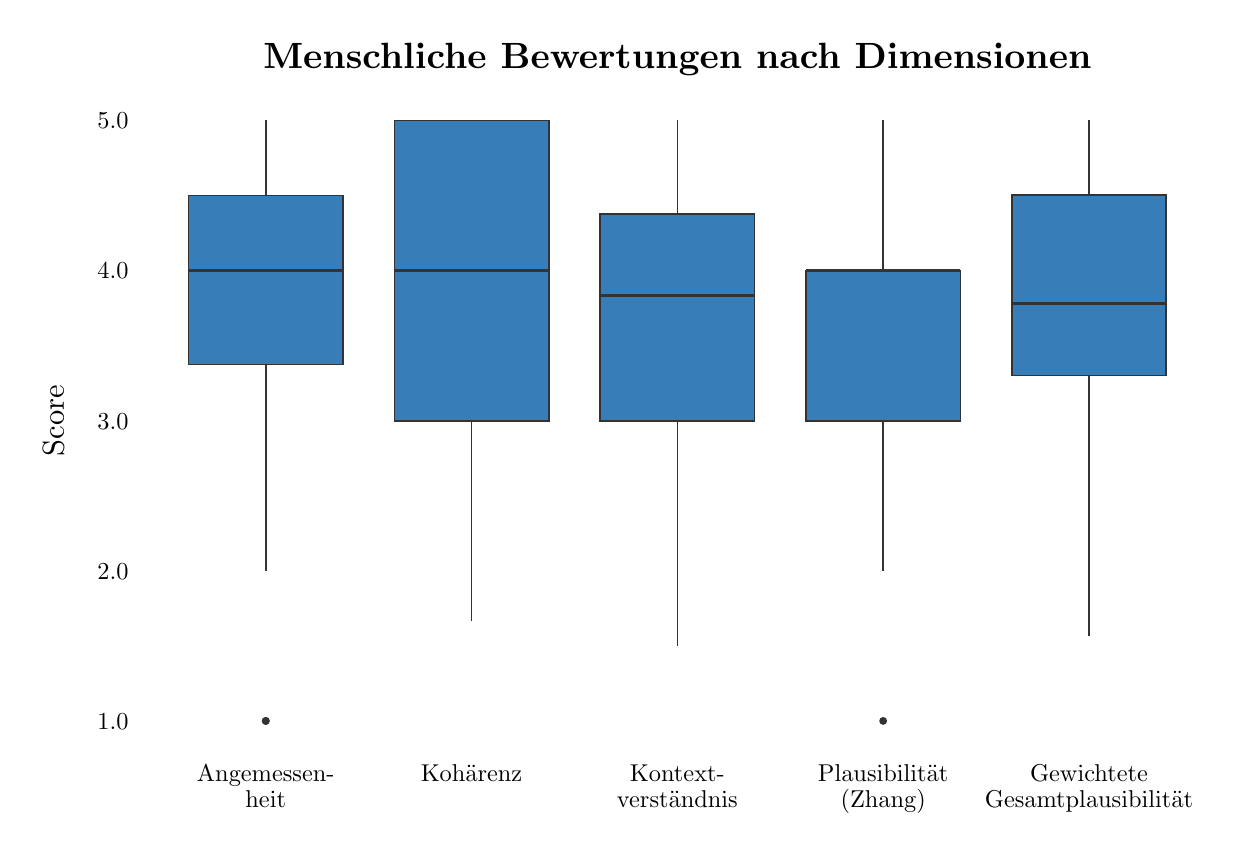
\begin{tikzpicture}[x=1pt,y=1pt]
\definecolor{fillColor}{RGB}{255,255,255}
\path[use as bounding box,fill=fillColor,fill opacity=0.00] (0,0) rectangle (433.62,289.08);
\begin{scope}
\path[clip] (  0.00,  0.00) rectangle (433.62,289.08);
\definecolor{fillColor}{RGB}{255,255,255}

\path[fill=fillColor] (  0.00,  0.00) rectangle (433.62,289.08);
\end{scope}
\begin{scope}
\path[clip] ( 41.41, 27.73) rectangle (428.12,266.40);
\definecolor{drawColor}{gray}{0.20}
\definecolor{fillColor}{gray}{0.20}

\path[draw=drawColor,line width= 0.4pt,line join=round,line cap=round,fill=fillColor] ( 86.03, 38.57) circle (  1.21);

\path[draw=drawColor,line width= 0.4pt,line join=round,line cap=round,fill=fillColor] ( 86.03, 38.57) circle (  1.21);

\path[draw=drawColor,line width= 0.6pt,line join=round] ( 86.03,228.43) -- ( 86.03,255.56);

\path[draw=drawColor,line width= 0.6pt,line join=round] ( 86.03,167.41) -- ( 86.03, 92.82);
\definecolor{fillColor}{RGB}{55,126,184}

\path[draw=drawColor,line width= 0.6pt,fill=fillColor] ( 58.14,228.43) --
	( 58.14,167.41) --
	(113.91,167.41) --
	(113.91,228.43) --
	( 58.14,228.43) --
	cycle;

\path[draw=drawColor,line width= 1.1pt] ( 58.14,201.31) -- (113.91,201.31);

\path[draw=drawColor,line width= 0.6pt,line join=round] (160.39,255.56) -- (160.39,255.56);

\path[draw=drawColor,line width= 0.6pt,line join=round] (160.39,147.06) -- (160.39, 74.74);

\path[draw=drawColor,line width= 0.6pt,fill=fillColor] (132.51,255.56) --
	(132.51,147.06) --
	(188.28,147.06) --
	(188.28,255.56) --
	(132.51,255.56) --
	cycle;

\path[draw=drawColor,line width= 1.1pt] (132.51,201.31) -- (188.28,201.31);

\path[draw=drawColor,line width= 0.6pt,line join=round] (234.76,221.65) -- (234.76,255.56);

\path[draw=drawColor,line width= 0.6pt,line join=round] (234.76,147.06) -- (234.76, 65.70);

\path[draw=drawColor,line width= 0.6pt,fill=fillColor] (206.88,221.65) --
	(206.88,147.06) --
	(262.65,147.06) --
	(262.65,221.65) --
	(206.88,221.65) --
	cycle;

\path[draw=drawColor,line width= 1.1pt] (206.88,192.27) -- (262.65,192.27);
\definecolor{fillColor}{gray}{0.20}

\path[draw=drawColor,line width= 0.4pt,line join=round,line cap=round,fill=fillColor] (309.13, 38.57) circle (  1.21);

\path[draw=drawColor,line width= 0.6pt,line join=round] (309.13,201.31) -- (309.13,255.56);

\path[draw=drawColor,line width= 0.6pt,line join=round] (309.13,147.06) -- (309.13, 92.82);
\definecolor{fillColor}{RGB}{55,126,184}

\path[draw=drawColor,line width= 0.6pt,fill=fillColor] (281.24,201.31) --
	(281.24,147.06) --
	(337.02,147.06) --
	(337.02,201.31) --
	(281.24,201.31) --
	cycle;

\path[draw=drawColor,line width= 1.1pt] (281.24,201.31) -- (337.02,201.31);

\path[draw=drawColor,line width= 0.6pt,line join=round] (383.50,228.66) -- (383.50,255.56);

\path[draw=drawColor,line width= 0.6pt,line join=round] (383.50,163.34) -- (383.50, 69.31);

\path[draw=drawColor,line width= 0.6pt,fill=fillColor] (355.61,228.66) --
	(355.61,163.34) --
	(411.39,163.34) --
	(411.39,228.66) --
	(355.61,228.66) --
	cycle;

\path[draw=drawColor,line width= 1.1pt] (355.61,189.56) -- (411.39,189.56);
\end{scope}
\begin{scope}
\path[clip] (  0.00,  0.00) rectangle (433.62,289.08);
\definecolor{drawColor}{RGB}{0,0,0}

\node[text=drawColor,anchor=base east,inner sep=0pt, outer sep=0pt, scale=  0.88] at ( 36.46, 35.54) {1.0};

\node[text=drawColor,anchor=base east,inner sep=0pt, outer sep=0pt, scale=  0.88] at ( 36.46, 89.79) {2.0};

\node[text=drawColor,anchor=base east,inner sep=0pt, outer sep=0pt, scale=  0.88] at ( 36.46,144.03) {3.0};

\node[text=drawColor,anchor=base east,inner sep=0pt, outer sep=0pt, scale=  0.88] at ( 36.46,198.28) {4.0};

\node[text=drawColor,anchor=base east,inner sep=0pt, outer sep=0pt, scale=  0.88] at ( 36.46,252.53) {5.0};
\end{scope}
\begin{scope}
\path[clip] (  0.00,  0.00) rectangle (433.62,289.08);
\definecolor{drawColor}{RGB}{0,0,0}

\node[text=drawColor,anchor=base,inner sep=0pt, outer sep=0pt, scale=  0.88] at ( 86.03, 16.71) {Angemessen-};

\node[text=drawColor,anchor=base,inner sep=0pt, outer sep=0pt, scale=  0.88] at ( 86.03,  7.21) {heit};

\node[text=drawColor,anchor=base,inner sep=0pt, outer sep=0pt, scale=  0.88] at (160.39, 16.71) {Kohärenz};

\node[text=drawColor,anchor=base,inner sep=0pt, outer sep=0pt, scale=  0.88] at (234.76, 16.71) {Kontext-};

\node[text=drawColor,anchor=base,inner sep=0pt, outer sep=0pt, scale=  0.88] at (234.76,  7.21) {verständnis};

\node[text=drawColor,anchor=base,inner sep=0pt, outer sep=0pt, scale=  0.88] at (309.13, 16.71) {Plausibilität};

\node[text=drawColor,anchor=base,inner sep=0pt, outer sep=0pt, scale=  0.88] at (309.13,  7.21) {(Zhang)};

\node[text=drawColor,anchor=base,inner sep=0pt, outer sep=0pt, scale=  0.88] at (383.50, 16.71) {Gewichtete};

\node[text=drawColor,anchor=base,inner sep=0pt, outer sep=0pt, scale=  0.88] at (383.50,  7.21) {Gesamtplausibilität};
\end{scope}
\begin{scope}
\path[clip] (  0.00,  0.00) rectangle (433.62,289.08);
\definecolor{drawColor}{RGB}{0,0,0}

\node[text=drawColor,rotate= 90.00,anchor=base,inner sep=0pt, outer sep=0pt, scale=  1.10] at ( 13.08,147.06) {Score};
\end{scope}
\begin{scope}
\path[clip] (  0.00,  0.00) rectangle (433.62,289.08);
\definecolor{drawColor}{RGB}{0,0,0}

\node[text=drawColor,anchor=base,inner sep=0pt, outer sep=0pt, scale=  1.32] at (234.76,274.47) {\bfseries Menschliche Bewertungen nach Dimensionen};
\end{scope}
\end{tikzpicture}
